\documentclass[a4paper,12pt]{article}
\usepackage{amsmath, amssymb, amsfonts, mathtools}
\usepackage[margin=1in, includefoot]{geometry}

%Figures ve Graph Tool Packages
\usepackage{graphicx, float}
\usepackage{pgfplots}
\usepackage{tikz}
\usepackage{xcolor}


%Table Packages
\usepackage{array}
\usepackage{caption}
\usepackage{enumitem}

%Header ve Footer Packages/Settings
\usepackage{fancyhdr}
\pagestyle{fancy}
\fancyhead{}
\fancyfoot{}
\fancyfoot[R]{\thepage}
\renewcommand{\headrulewidth}{0pt}
\setlength{\parindent}{0pt}


\begin{document}

	\begin{titlepage}
		\begin{center}
			
			\vspace*{3cm}
			\huge\bfseries İstatistiksel Kalite Kontrol \\Dönem Ödevi
			\vspace*{6cm}
			\begin{center}
				\huge\bfseries{"Homework 9" İçin\\ İstatistiksel Hesaplamalar}\\
				\text{\large Berkay Coşgun}\\
				\textsc{\small 2021285013}\\
			\end{center}
		 	
		 	\vspace*{\fill}
			
			\text{\small 2024-2025, Güz}		 	
		 			
		\end{center}
	\end{titlepage}
	
	\begin{quote}
		
		\vspace*{\fill}
		\begin{center}
			Bu ödevin hazırlanmasında \LaTeX\ kullanılmıştır.
		\end{center}
		\vspace*{8cm}
		\textbf{Özet}\\
		Soruda bize verilen verilerde, bir "dry bleach" ürününün net ağırlık verilerine dayalı istatistiksel kalite kontrol süreci yapılmıştır. 20 örneklem ve her örneklemde 5 gözlemden oluşan veri seti üzerinde $\bar{X}$ ve $S$ Kontrol Kartları'nın istatistikleri ile popülasyon parametreleri tahmin edilmiş ve bu bilgilerle süreç yeterliliği incelenmiştir.
		
		
		\vspace*{\fill}
		
		\pagenumbering{roman}
		\cleardoublepage
	
	\end{quote}
	
	\begin{quote}
		\tableofcontents
		\cleardoublepage
	\end{quote}
	
		
	%Sayfa Numaraları Düzeni
	\pagenumbering{arabic}
	\setcounter{page}{1}
	

\section{"Homework 9" Tablo ve Sorular}

	Soruya ilk yaklaşım olarak, bize verilen 5 elemanlı ve 20 deneyden oluşan Table 6E.6 verilerini kullanarak, ilerleyen hesaplamalarımızda gerekli olan istatistikleri önceden elde edebilmek amacıyla 'Table 6E.6.1' adlı yeni bir tablo yapılacaktır.
	
	\renewcommand{\arraystretch}{1}
	
	\begin{table}[h!]
		\centering
		\caption*{\bfseries Table 6E.6}
		\begin{tabular}{|c|c|c|c|c|c|}
			\hline
			\textbf{Sample} & \textbf{$x_1$} & \textbf{$x_2$} & \textbf{$x_3$} & \textbf{$x_4$} & \textbf{$x_5$} \\ \hline
			1 & 15,8 & 16,3 & 16,2 & 16,1 & 16,6 \\ \hline
			2 & 16,3 & 15,9 & 15,9 & 16,2 & 16,4 \\ \hline
			3 & 16,1 & 16,2 & 16,5 & 16,4 & 16,3 \\ \hline
			4 & 16,3 & 16,2 & 15,9 & 16,4 & 16,2 \\ \hline
			5 & 16,1 & 16,1 & 16,4 & 16,5 & 16,0 \\ \hline
			6 & 16,1 & 15,8 & 16,7 & 16,6 & 16,4 \\ \hline
			7 & 16,1 & 16,3 & 16,5 & 16,1 & 16,5 \\ \hline
			8 & 16,2 & 16,1 & 16,2 & 16,1 & 16,3 \\ \hline
			9 & 16,3 & 16,2 & 16,4 & 16,3 & 16,5 \\ \hline
			10 & 16,6 & 16,3 & 16,4 & 16,1 & 16,5 \\ \hline
			11 & 16,2 & 16,4 & 15,9 & 16,3 & 16,4 \\ \hline
			12 & 15,9 & 16,6 & 16,7 & 16,2 & 16,5 \\ \hline
			13 & 16,4 & 16,1 & 16,6 & 16,4 & 16,1 \\ \hline
			14 & 16,5 & 16,3 & 16,2 & 16,3 & 16,4 \\ \hline
			15 & 16,4 & 16,1 & 16,3 & 16,2 & 16,2 \\ \hline
			16 & 16,0 & 16,2 & 16,3 & 16,3 & 16,2 \\ \hline
			17 & 16,4 & 16,2 & 16,4 & 16,3 & 16,2 \\ \hline
			18 & 16,0 & 16,2 & 16,4 & 16,5 & 16,1 \\ \hline
			19 & 16,4 & 16,0 & 16,3 & 16,4 & 16,4 \\ \hline
			20 & 16,4 & 16,4 & 16,5 & 16,0 & 15,8 \\ \hline
		\end{tabular}
		\caption*{The net weight (in oz) of a dry bleach product}
		\label{tab:sample-data}
	\end{table}
	
	\begin{enumerate}[label=(\alph*)]
	 
\item
 The net weight (in oz) of a dry bleach product is to be monitored by X and S control charts using a sample size of n = 5. Data for 20 preliminary samples are shown in Table 6E.6.  
\item
 Set up and S control charts using these data. Does the process exhibit statistical control? 


\item
Estimate the process mean and standard deviation. 


\item
Does fill weight seem to follow a normal distribution? 


\item
If the specifications are at 16.2 ± 0.5, what conclusions would you draw about process capability? 


\item
What fraction of containers produced by this process is likely to be below the lower specification limit of 15.7 oz? 
	\end{enumerate}
	





\section{İlk Hesaplamalar}

Soruya ilk yaklaşım olarak, bize verilen 5 elemanlı ve 20 deneyden oluşan Table 6E.6 verilerini kullanarak, ilerleyen hesaplamalarımızda gerekli olan istatistikleri önceden elde edebilmek amacıyla 'Table 6E.6.1' adlı yeni bir tablo oluşturacağız ve soru çözümlerinde ona başvuracağız. 

\renewcommand{\arraystretch}{1.2}

\begin{table}[h!]
	\centering
	\caption*{\bfseries Table 6E.6.1}
	\begin{tabular}{|c|c|c|c|}
		\hline
		\textbf{Sample} & \textbf{$\bar{x_i}$} & \textbf{$s_i$} & \textbf{$R_i$} \\
		\hline
		1 & 16,2000 & 0,2608 & 0,8000 \\
		2 & 16,1400 & 0,2059 & 0,5000 \\
		3 & 16,3000 & 0,1414 & 0,4000 \\
		4 & 16,2000 & 0,1673 & 0,5000 \\
		5 & 16,2200 & 0,1939 & 0,5000 \\
		6 & 16,3200 & 0,3311 & 0,9000 \\
		7 & 16,3000 & 0,1789 & 0,4000 \\
		8 & 16,1800 & 0,0748 & 0,2000 \\
		9 & 16,3400 & 0,1020 & 0,3000 \\
		10 & 16,3800 & 0,1720 & 0,5000 \\
		11 & 16,2400 & 0,1855 & 0,5000 \\
		12 & 16,3800 & 0,2926 & 0,8000 \\
		13 & 16,3200 & 0,1939 & 0,5000 \\
		14 & 16,3400 & 0,1020 & 0,3000 \\
		15 & 16,2400 & 0,1020 & 0,3000 \\
		16 & 16,2000 & 0,1095 & 0,3000 \\
		17 & 16,3000 & 0,0894 & 0,2000 \\
		18 & 16,2400 & 0,1855 & 0,5000 \\
		19 & 16,3000 & 0,1549 & 0,4000 \\
		20 & 16,2200 & 0,2713 & 0,7000 \\
		\cline{2-4}
	&$\bar{\bar{x}}=16,2680$&$\bar{s}=0,175$7&$\bar{R}=0,475$\\
		\hline
	\end{tabular}
	\caption*{}
\end{table}

Her bir deneydeki sabit gözlem sayısı olan n=5 bilgisi ile ihtiyacımız olacak tüm katsayıların sayısal değerlerini biliyoruz.  

Tablodaki değerlerin hesaplaması için: 

\begin{enumerate}[label=\Roman{enumi}.]
	

\item
$\bar{x} = \frac{1}{20}\sum_{i=1}^{20}\bar{x_i} = \frac{1}{20}(325,3600) = 16,268$
\item
$\bar{s}=\frac{1}{20}\sum _{i=1}^{20}\bar{s_i}=\frac{1}{20}\left(3,5147\right)=0,1757$
\item
$\bar{R}=\frac{1}{m}\sum _{i=1}^{20}R_i=\frac{1}{20}\left(9,500\right)=0,475$

\end{enumerate}

\cleardoublepage

Bu bilgilerin bize sundukları: 

\begin{enumerate}[label=\Roman{enumi}.]
	\item
	Her bir deney için farklı olan ortalamanın, toplam deney sayısına göre ortalaması 
	\item
	Her bir deney için farklı olan standart sapmalarının, toplam deney sayısına göre ortalaması 
	\item
	Her bir deneydeki en uç değerlerin farkının, toplam deney sayısına göre ortalaması 
\end{enumerate}

Öncelikle, $\bar{X}$ kontrol kartının grafiğini çizmeye çalışacağız. 

\begin{itemize}
	\item
	\centering
	$UCL=\bar{\bar{x}}+A_3\cdot \ \bar{s}=16,2680+\left(0,680\ast 0,1757\right)=16,5188$
	\item
	$CL\ =\ \bar{s}\ =\ 16,2680$
	\item
	$LCL=\bar{\bar{x}}-A_3\cdot \bar{s}=16,2680-\left(0,680\ast 0,1757\right)=16,0172$
\end{itemize}




\begin{figure}[ht]
	\centering
	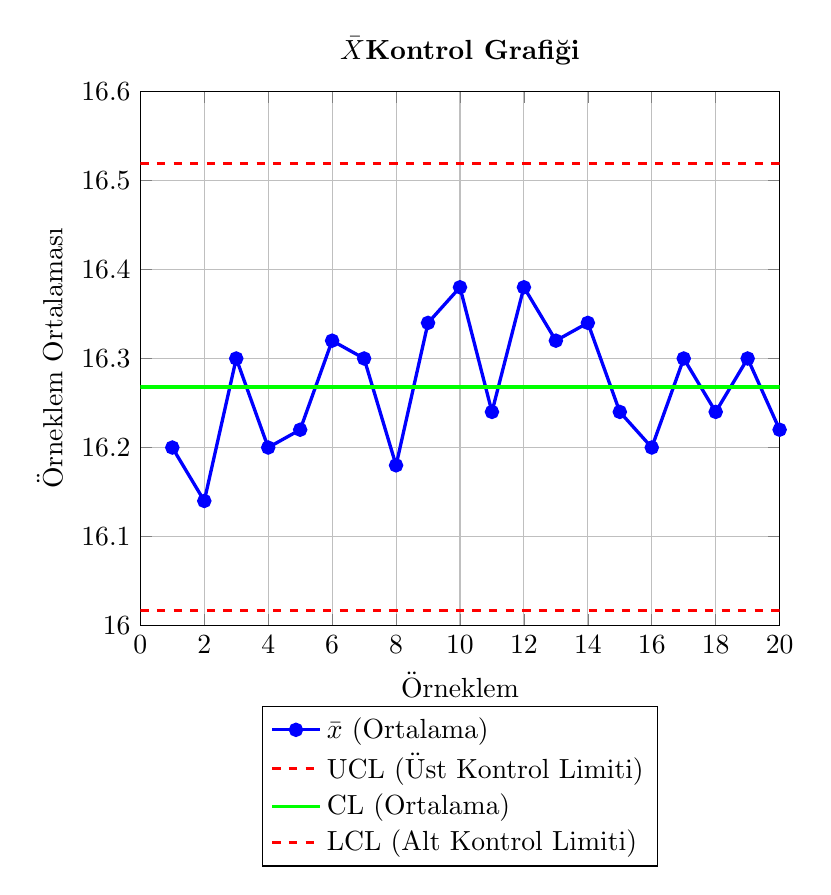
\begin{tikzpicture}
		\begin{axis}[
			title={\bfseries $\bar{X}$Kontrol Grafiği},
			xlabel={Örneklem},
			ylabel={Örneklem Ortalaması},
			xmin=0, xmax=20,
			ymin=16, ymax=16.6,
			grid=both,
			    legend style={at={(0.5,-0.15)}, anchor=north},
			    legend cell align=left,
			    legend entries={},
			width=0.8\textwidth,
			]

			\addplot[
			color=blue,
			mark=*,
			very thick
			] coordinates {
				(1, 16.2) (2, 16.14) (3, 16.3) (4, 16.2) (5, 16.22) 
				(6, 16.32) (7, 16.3) (8, 16.18) (9, 16.34) (10, 16.38)
				(11, 16.24) (12, 16.38) (13, 16.32) (14, 16.34) (15, 16.24) 
				(16, 16.2) (17, 16.3) (18, 16.24) (19, 16.3) (20, 16.22)
			};
			\addlegendentry{$\bar{x}$ (Ortalama)}
			
			% UCL çizgisi
			\addplot[
			color=red,
			dashed,
			very thick
			] coordinates {
				(0, 16.5188) (20, 16.5188)
			};
			\addlegendentry{UCL (Üst Kontrol Limiti)}
			
			% CL çizgisi
			\addplot[
			color=green,
			very thick
			] coordinates {
				(0, 16.2680) (20, 16.2680)
			};
			\addlegendentry{CL (Ortalama)}
			
			% LCL çizgisi
			\addplot[
			color=red,
			dashed,
			very thick
			] coordinates {
				(0, 16.0172) (20, 16.0172)
			};
			\addlegendentry{LCL (Alt Kontrol Limiti)}
			
		\end{axis}
	\end{tikzpicture}
	\caption*{}
\end{figure}


ilk dikkat çeken pattern, ortalama etrafında salınım yapan gözlemlerdir. Evet, istatistiksel olarak bu sürecin “yeterli” olduğunu söyleyebiliriz. Sebebini ise “kontrol limitlerine ulaşan herhangi bir gözlem (phase 2) gerçekleşmemiş” olarak açıklayabiliriz. Grafiğin yaptığı salınım, özellikle birbiri ardına olan gözlemlerdeki ortalama farklılıkları, süreci inceleyen bizlere şu noktaların düşünülmesi gerektiği hakkında bazı fikirler verir: 

\begin{enumerate}[label=\Roman{enumi}.]
	\item 
	Örneğimizdeki süreçte ağırlığı takip edilen dry bleach’ı işleten ve ambalajlayan makinelerin kalibrasyonunda bir sıkıntı oluyor veya fabrikanın üretim bandında prosedür dışı beklenmeyen bir olay gerçekleşiyor olabilir. 
	\item 
	Eğer makineler bir operatör yardımı ile çalıştırılıyor ise, birbirinden farklı çalışma stillerine sahip olan çalışanların yarattığı bir sorun olabilir. Çalışan ve gözlemler arasında bir bağlantı var mı diye bakılmalıdır. 
	\item 
	Süreç sürekli incelendiği için yapılan denemeler belki de birbirini etkiliyor, üretim hattı düzgün koşullar ile incelenmiyor veya yapılan gözlemler birbirinden farklı makineler, departmanlar veya koşullar arasında yapıldığından deney aynı çıktıları sağlayamıyor olabilir. \\
	
	Xbar Kontrol Kart'ı ve süreç hakkındaki yorumlamalardan sonra artık S Kontrol Kartı’nın kontrol limitlerini hesaplamaya, grafiğini çizmeye ve ardından (a) şıkkı için nasıl yorumlanması gerektiği hakkında konuşulacaktır. 
	
\end{enumerate}


\section{A Şıkkı}

Kontrol limitleri için daha önceden hesapladığımız ortalama örneklem standart sapması ve n=5 için olan katsayıları kullanarak hesaplama yapıldığında: 

\begin{itemize}
	\centering
	\item 
	$UCL=B_4 \bar{s}=(2,089 \cdot 0,1757)=0,3671$
	\item
	$CL=\bar{s}=0,1757$
	\item
	$LCL=B_3 {s}=(0 \cdot 0,1757)=0$
\end{itemize}


Süreç aslında “istatistiksel olarak kontrol altındadır” ama incelenilmesi gereken bazı noktalar vardır.\\

S Kontrol Kart'ı tıpkı $\bar{X}$ Kontrol Kartı'nda da söylendiği gibi operatör farklılıkları, makine kalibre sıkıntıları, standartize edilmemiş üretim gibi sorunlara sahip olabilir. Ayrıca bu grafik, yapılan her bir gözlemdeki ürünlerin gramaj değişikliğin kontrol limitlerinin altında dahi olsa süreçteki bir düzensizliği ortaya koymaktadır.\\

Bu süreç özelinden gidildiğinde $\bar{X}$ Kontrol Kartı ile S Kontrol Kartları'nın en büyük farkı ise, birisinin her bir gözlemdeki “ortalamamız ne?” sorusuna cevap vermeye çalışırken diğerinin ise her bir gözlemde “tutarlılığımız ne kadar?”  sorusuna cevap vermeye çalışmasıdır. \\

Bir örnek ile anlatılmak istenilirse, 2 kiloluk ürün ile 10 kiloluk ürünün ortalaması 6 kilodur fakat 5 kiloluk ve 7 kiloluk iki ürününde ortalaması da 6 kilo olacaktır. İki durumu birbirinden ayırabilmek ve sürecin tutarlı, ürünlerin aynı kalitede olabilmesi için gözlemlerin standart sapmalarının düşük olmasını beklemek kesinlikle normal ve istenilmesi gerekilen bir durumdur.\\

\begin{figure}[ht]
	\centering
	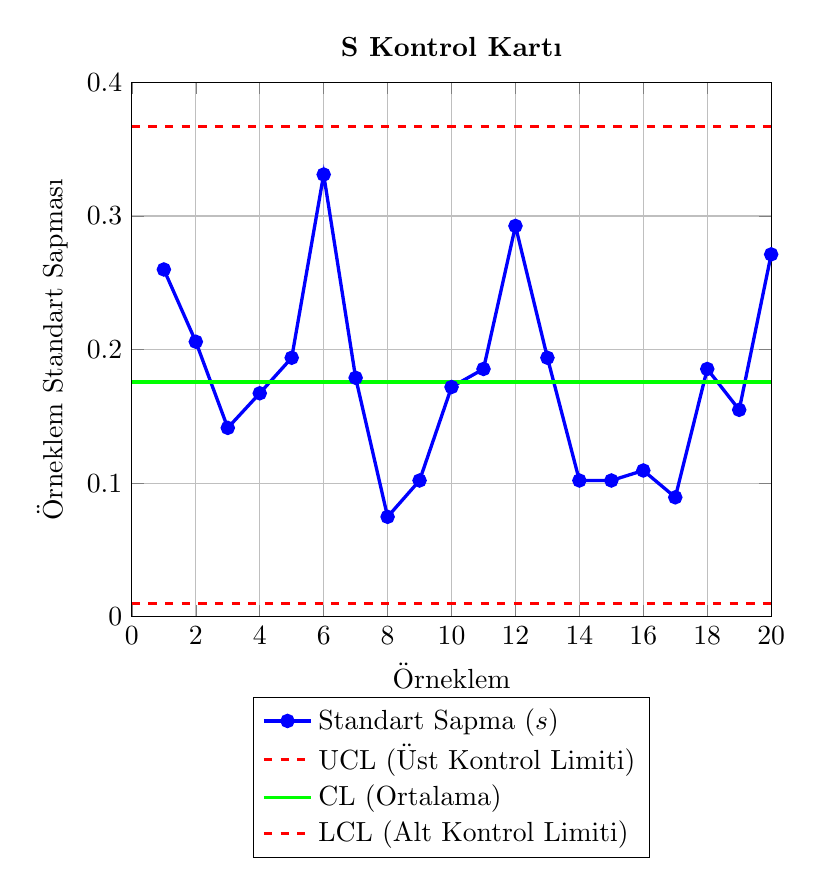
\begin{tikzpicture}
		\begin{axis}[
			title={\bfseries S Kontrol Kartı},
			xlabel={Örneklem},
			ylabel={Örneklem Standart Sapması},
			xmin=0, xmax=20,
			ymin=0, ymax=0.4,
			grid=both,
			yticklabel style={/pgf/number format/fixed},
			legend style={at={(0.5,-0.15)}, anchor=north}, % legend'ı alt tarafa yerleştirme
			legend cell align=left,
			legend entries={},
			width=0.8\textwidth
			]
			% Standart Sapma (s) verisi
			\addplot[
			color=blue,
			mark=*,
			very thick
			] coordinates {
				(1, 0.26) (2, 0.2059) (3, 0.1414) (4, 0.1673) (5, 0.1939) 
				(6, 0.3311) (7, 0.1789) (8, 0.0748) (9, 0.1020) (10, 0.1720)
				(11, 0.1855) (12, 0.2926) (13, 0.1939) (14, 0.1020) (15, 0.1020) 
				(16, 0.1095) (17, 0.0894) (18, 0.1855) (19, 0.1549) (20, 0.2713)
			};
			\addlegendentry{Standart Sapma ($s$)}
			
			% UCL çizgisi
			\addplot[
			color=red,
			dashed,
			very thick
			] coordinates {
				(0, 0.3671) (20, 0.3671)
			};
			\addlegendentry{UCL (Üst Kontrol Limiti)}
			
			% CL çizgisi
			\addplot[
			color=green,
			very thick
			] coordinates {
				(0, 0.1757) (20, 0.1757)
			};
			\addlegendentry{CL (Ortalama)}
			
			% LCL çizgisi
			\addplot[
			color=red,
			dashed,
			very thick
			] coordinates {
				(0, 0.0100) (20, 0.0100)
			};
			\addlegendentry{LCL (Alt Kontrol Limiti)}
			
		\end{axis}
	\end{tikzpicture}
	\caption*{}
\end{figure}


Ödevin bu kısmına kadar yapılan (a) şıkkının S Kontrol Kartı'nın yorumlaması yapıldıktan sonra artık (b) şıkkı hakkında yorumlamalar yapılacaktır.

\cleardoublepage



\section{B Şıkkı}

Sürecin örneklem ortalamasını tahmin etmek için $\bar{\bar{x}}$ kullanılabilir ve değeri $16,2680$ olacaktır.\\

Süreç standart sapmasını hesaplamak için hem örneklem standart sapmasını hem de range değerleri ile hesaplamalar yapıldığında,\\


${\hat{\sigma}}_x = \frac{\bar{s}}{c_4} = \frac{0,1757}{0,9400} = 0,1869$
ve
${\hat{\sigma}}_x = \frac{\bar{R}}{d_2} = \frac{0,475}{2,326} = 0,2042$\\

Birbirine yakın ama aynı olmayan iki farklı süreç standart sapması hesaplandı. Bunun sebebi örneklem boyutu, seçilen örneklem istatistiğin ve yanlılık düzeltme katsayıları arasındaki farktır.

\subsection{Tahmincilerin yansızlığı ve beklenen değer operatörü ile hesaplamalar}

Örneklem ortalaması ve varyansı olan $\bar{x}$ ve $s^{2}$ popülasyon ortalaması ve varyansı olan $\mu$ ve $\sigma^{2}$ için yansız bir tahmincidir.\\

İstatistiksel olarak $E(\bar{x}) = \mu$ ve $E(\bar{s^{2}}) = \sigma^{2}$ şeklinde gösterilir. Çünkü $T(X) = \hat{\theta}$ eğer ki $\theta$ için bir tahminci ise o zaman bu tahmincinin $\theta$ için sapması, farkı ya da yanlılığı $bias(\hat{\theta}) = E_{\theta}(\hat{\theta}) - \theta$ olacaktır. Yani, yanlılık için beklenen değer ile hesaplamalar yapmamız gerekmektedir.\\

Fakat, örneklem standart sapması olan $s$ popülasyon standart sapması olan $\sigma$ için yansız bir kesirci değildir. Bu sebeple $E(s) \neq \sigma$ olacaktır.

Örneklem standart sapmasının neden popülasyon standart sapmasına eşit olmadığını ispatlamak için Jensen’s İnequality ile işlemler yapalım.\\

Eğer $f : I \to \mathbb{R}$ ve tüm $x \in I$ için $f''(x) \le 0$ konkav bir fonksiyon ve $X$ integrallenebilir bir rasgele değişken olmak üzere, 
\begin{itemize}[label*={}]
	\item 
	Jensen's Inequality $E(f(X)) \le f(E(X)) $
	\item 
	$f(s) = \sqrt{s^{2}}$
	\item
	$E(\sqrt{s^{2}}) \le \sqrt{E(s^{2})}$ ve \text{$E(s^{2}) = \sigma^{2}$, $\sqrt{\sigma^{2}} = \sigma$ olduğu için}
	\item 
	$E(s) \le \sigma$
\end{itemize}

Bu ispattan da anlaşılabileceği gibi, örneklem varyansının karekökü popülasyon varyansına her zaman eşit değildir. Sadece parametrenin gerçek değerine eşit olursa birbirlerine eşit olabilirler. Bu sebeplerden ötürü $E(s) = \sigma$ doğru bir ifade değildir. Bu yüzden örneklem boyutu $2\le n \le25$ olan süreçlerde düzeltme faktörü olarak kullanılan $c_4$, popülasyon parametresini için daha doğru sonuçlar verir. $E(s)=\left(\frac{2}{n-1}\right)^{\frac{1}{2}}\cdot \frac{\Gamma (n/2)}{\Gamma(\frac{n-1}{2})}\cdot \sigma =c_4\cdot \sigma$ ve populasyon tahmincisi olarak $\hat{\sigma }=\frac{\bar{s}}{c_4}$ şeklinde hesaplanır\\

\section{C Şıkkı}

Bu kısmına kadar yapılan süreç ortalaması ve süreç standart sapması hakkındaki yorumlamalardan sonra artık yeni soru hakkında yorumlamalar yapılacaktır.\\

İlk öncelikle gözlemlenen ağırlıkların histogram grafiğini çizelim. 

\begin{center}
	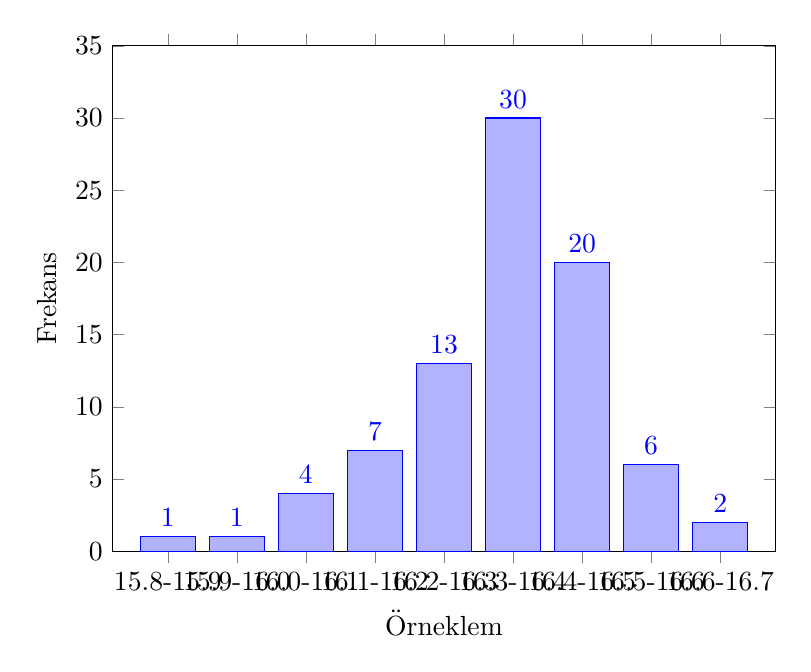
\begin{tikzpicture}
		\begin{axis}[
			ybar,
			bar width=0.7cm,
			width=10cm,
			height=8cm,
			xlabel={Örneklem},
			ylabel={Frekans},
			symbolic x coords={15.8-15.9, 15.9-16.0, 16.0-16.1, 16.1-16.2, 16.2-16.3, 16.3-16.4, 16.4-16.5, 16.5-16.6, 16.6-16.7},
			xtick=data,
			nodes near coords,
			ymin=0,
			ymax=35
			]
			\addplot coordinates {
				(15.8-15.9, 1)
				(15.9-16.0, 1)
				(16.0-16.1, 4)
				(16.1-16.2, 7)
				(16.2-16.3, 13)
				(16.3-16.4, 30)
				(16.4-16.5, 20)
				(16.5-16.6, 6)
				(16.6-16.7, 2)
			};
		\end{axis}
	\end{tikzpicture}
\end{center}

Süreç boyunca kaydedilen tüm ağırlıkların normal dağılıma sahip olduğunu anlamanın en basit yolu histogram grafiğinin çan eğrisi ile kıyaslamaktır. Bu, dağılımın normal olup olmadığını anlamamız için şimdilik yeterlidir. Histograma göre söylenebilir ki evet, veriler normal dağılıma yakındırlar.



\section{D Şıkkı}

(c) Şıkkı’nın histogram yorumundan sonra (d) şıkkı hakkında yorumlamalar yapılacaktır.\\

Process Capability Ratio $C_p$ için 3 genel durum vardır.
\begin{itemize}[label*={}]
	\item 
	$C_p \le 1$ süreç yetersizdir
	\item 
	$C_p = 1$ süreç yeterlidir ama tolere edilebilir değildir, sınırdadır
	\item 
	$C_p \ge 1$ süreç yeterlidir\\
	\end{itemize}
	
	Süreç yeterliliği için bir tahminci ($\hat{\sigma_x}$) kullandığımız için $\hat{C_p}$ doğru notasyondur.
\begin{itemize}[label*={}]
	\item
	$\hat{C}_p = \frac{USL-LSL}{6\hat{\sigma_x}} = \frac{0,5-(-0,5)}{6*(0,2042)} = \frac{1}{1,2252} = 0,8161$ olarak bulunur.

 \end{itemize}

	
$C_p$ için süreç yetersizdir. Kontrol kartları tolerans limitlerini aşmasa da bu durumu bir noktada destekliyordu.\\

\section{E Şıkkı}

Sayfanın devamında (d) şıkkının süreç yeterliliği yorumundan sonra (e) şıkkı hakkındaki yorumlamalar yapılacaktır.\\

Süreç boyunca elde edilen verilere göre 15,7 oz’dan daha az olma ihtimalinin hesaplanması için normal dağıldığını varsaydığımız bu süreci standart normale dönüştürüp, çan eğrisi altında kalan alana göre yüzde kaç ihtimal ile gerçekleşebileceğini inceleyeceğiz.

\begin{itemize}[label*={}]
	\item
	$P\left(x < \text{LSL}\right)$
	\item
	$P\left(\frac{x-\mu}{\hat\sigma_x} < \frac{\mu - \text{LSL}}{\hat\sigma_x}\right)$
	\item
	$P\left(Z < \frac{15,7-16,2680}{0,2042}\right)$
	\item
	$P\left(Z < \frac{-0.5680}{0.2042}\right)$
	\item
	$P\left(Z < -2,7815\right) \cong 0,0027$ olarak bulunur.
\end{itemize}

\%0,27 olasılık ile 15.7 oz ve daha aşağısında ürününün (dry bleach) bu üretimden çıkabilme olasılığını hesapladık.\\

\begin{center}
	
$X\ \sim \ N\left(16,2080\ \left(0,2042\right)^2\right)$ için grafik şu şekildedir.\\

\pgfplotsset{compat=1.18}
\pgfmathsetmacro{\mu}{16.2080}
\pgfmathsetmacro{\sigma}{0.2042	}
\pgfmathdeclarefunction{normal}{2}{%
	\pgfmathparse{1/(#2 * sqrt(2 * pi)) * exp(-((x - #1)^2) / (2 * #2^2))}%
}

\begin{tikzpicture}[scale=0.80]
	\begin{axis}[
		domain=15:17.5,
		samples=100,
		xlabel={$X$}, 
		ylabel={$f(x)$},
		axis lines=middle, 
		enlargelimits, 
		height=8cm, width=8cm,
		]
		
		\addplot[blue, thick]{normal(\mu, \sigma)};
		
	\end{axis}
\end{tikzpicture}
\\[0.25in]

$X\ \sim \ Z(0,1)$ için ise grafik bu şekildedir.

\pgfplotsset{compat=1.18}
\pgfmathdeclarefunction{normalpdf}{1}{%
	\pgfmathparse{1/(sqrt(2*pi))*exp(-(#1^2)/2)}%
}

\begin{tikzpicture}[scale=0.80]
	\begin{axis}[
		domain=-4:4,
		samples=100,
		axis lines=middle,
		enlargelimits,
		height=8cm, 
		width=12cm,
		grid style={dashed,gray!30},
		ylabel style={at={(axis description cs:-0.1,.5)},rotate=90,anchor=south},
		xtick={-3,-2,-1,0,1,2,3},
		ytick={0,0.1,0.2,0.3,0.4},
		ymax=0.45
		]
		\addplot[blue, thick] {normalpdf(x)};
		
	\end{axis}
\end{tikzpicture}
\end{center}




\section{Kaynaklar}


\renewcommand{\refname}{}

\begin{thebibliography}{}
	
	\hrule\vspace{0.5cm}
	
	\bibitem{referans1} Montgomery, Introduction to Statistical Quality Control (p. 110-251-351), Sixth Edition,
	
	\bibitem{referans2} Degroot, Probability and Statistics (p. 322-393), Third Edition
	
	\bibitem{referans3} David E. Giles, Unbiased Estimation of the Standard Deviation for Non-Normal Populations
	
	\bibitem{referans4} Billingsley, P. (2008). Probability and measure (p. 84-85), Second Edition
\end{thebibliography}

Bu \LaTeX\ metninin kaynak dosyalarını https://github.com/berkayscosgun/homework9 adresinden indirebilirsiniz.



\end{document}